\subsection{}
Total cost is the sum of total variable cost and total fixed cost.
\begin{equation}
    TC = TVC + TFC
\end{equation}
Or total cost is the sum of the labour and capital costs.\\
Total variable cost is worker wages multiplied by the number of workers.
\begin{figure}[H]
    \centering
    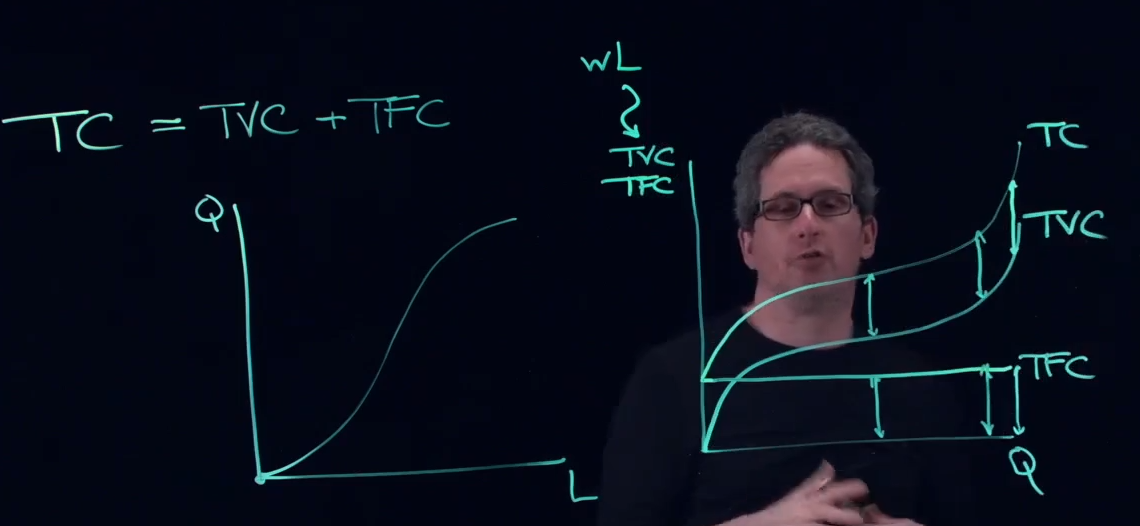
\includegraphics[width=0.5\textwidth]{Chapter7/TotalCost.png}
    \caption{Total Cost}
\end{figure}
\par
The average (total) cost, average variable cost and average fixed cost are found by drawing a linear line from the origin to the total curve.\\
The AC starts at infinity and decreases as the quantity increases.\\
The tangent point of TC must come after the tangent point of TVC.\\
AC and AVC never cross.\\
AFC decreases as quantity increases and can never be zero.
\begin{equation}
    AC = \frac{TC}{Q}
\end{equation}
\begin{equation}
    AVC = \frac{TVC}{Q}
\end{equation}
\begin{equation}
    AFC = \frac{TFC}{Q}
\end{equation}
\begin{equation}
    AC = AVC + AFC
\end{equation}
\par
Marginal cost is the cost of producing one more unit.
\begin{equation}
    MC = \frac{\Delta TC}{\Delta Q} = \frac{\Delta TVC}{\Delta Q}
\end{equation}
\begin{equation}
    MVC = \frac{\Delta TVC}{\Delta Q} = \frac{\Delta TC}{\Delta Q} - \frac{\Delta TFC}{\Delta Q}
\end{equation}
\begin{equation}
    MFC = \frac{\Delta TFC}{\Delta Q} = 0
\end{equation}
\begin{equation}
    MC = MVC
\end{equation}
\begin{figure}[H]
    \centering
    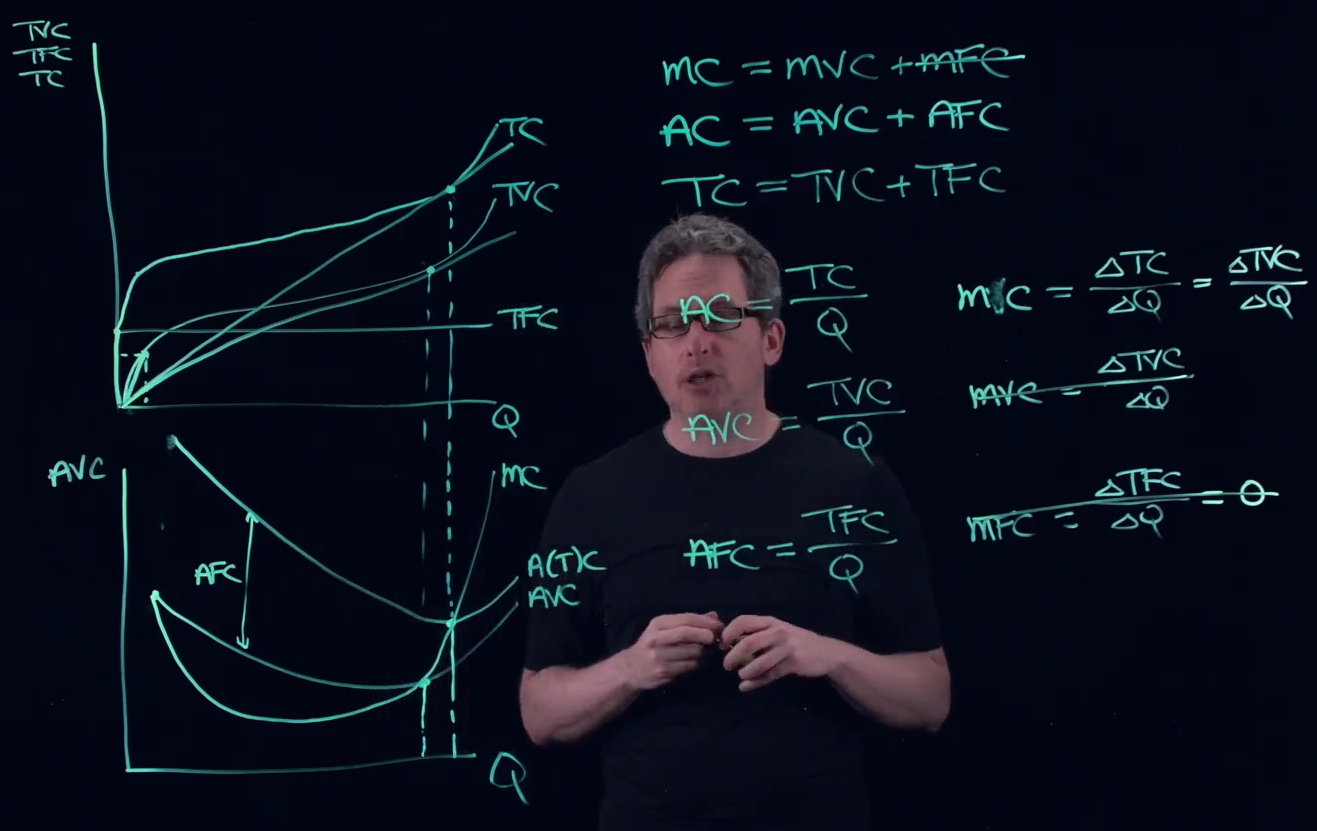
\includegraphics[width=0.5\textwidth]{Chapter7/MarginalCost.png}
    \caption{Average and Marginal Cost}
\end{figure}
\par
\begin{equation}
    MC = \frac{W}{\text{Marginal Product}(MP)}
\end{equation}
\begin{equation}
    MC = \frac{\Delta TC}{\Delta Q}
\end{equation}
\begin{equation}
    \frac{W}{MP} = \frac{W\Delta L}{\Delta Q} = \frac{\Delta TC}{\Delta Q}
\end{equation}
\begin{equation}
    AVC = \frac{W}{AP}
\end{equation}
This can also be represented in a table.
\begin{figure}[H]
    \centering
    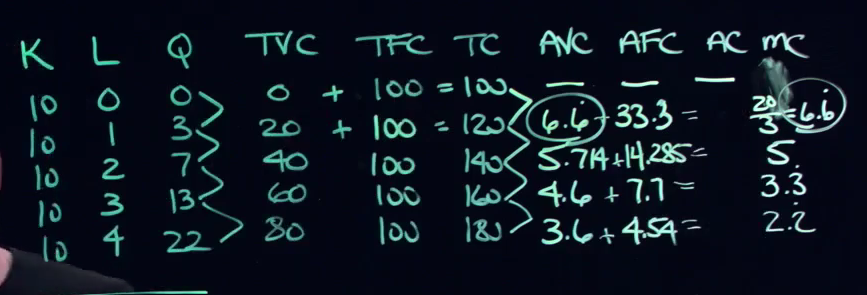
\includegraphics[width=0.5\textwidth]{Chapter7/CostTable.png}
    \caption{Cost Table}
\end{figure}
When AC is at minimum point, profits are maximized.